\vspace{-.2in}
\section{Introduction}
\label{section:introduction}


%Black holes are believed to be surrounded by a boundary called the event horizon, beyond which light can no longer escape the immense gravitational pull. \katie{previous sentance is awkward} 

High resolution celestial imaging is essential for progress in astronomy and physics. 
For example, imaging the plasma surrounding a black hole's event horizon at high resolution could help answer many important questions; 
%most notably, it may aid in unifying  the theories of general relativity and quantum mechanics. 
most notably, it may substantiate the existence of black holes~\cite{blackholesexist} as well as verify and test the effects of general relativity~\cite{nohairtheroem}.  
Recently, there has been an international effort to create an Event Horizon Telescope (EHT) capable of imaging a black hole's event horizon for the first time~\cite{doeleman2012jet, doeleman2008event}. The angular resolution necessary for this observation is at least an order of magnitude smaller than has been previously used to image radio sources~\cite{krichbaum2006sub}.
As measurements from the EHT become available, 
robust algorithms able to reconstruct images in this fine angular resolution regime will be necessary. 
%Advances from the computer vision community in statistical image models and super-resolution as well as sophisticated inference algorithms are invaluable to the success of these reconstruction methods~\cite{zoran2011learning}~\cite{glasner2009super}~\cite{freeman2002example}~\cite{levin2011efficient}. 

\begin{figure}[t!]
	\centering
	\subfigure[Telescope Locations]{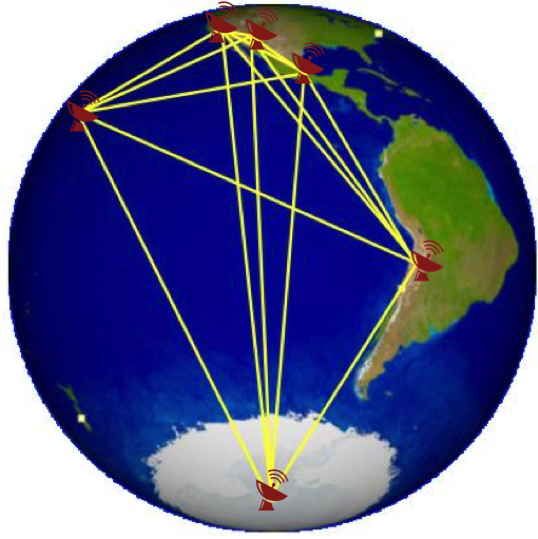
\includegraphics[width=0.45\linewidth]
		{world.png}}
	\subfigure[Spatial Frequency Coverage]{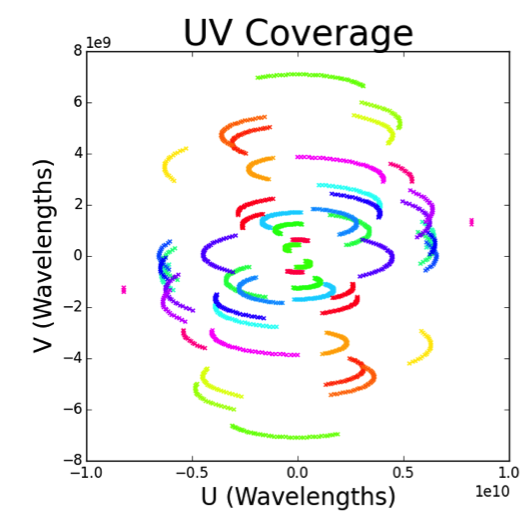
\includegraphics[width=0.5\linewidth]
		{uvcoverage.png}}
	\caption{ \footnotesize{{\bf Frequency Coverage:} (A) A sample of the telescope locations in the EHT. By observing a source over the course of a day, we obtain measurements corresponding to elliptical tracks in the source image's spatial frequency plane (B). These frequencies, $(u,v)$, are the projected baseline lengths orthogonal to a telescope pair's light of sight. Points of the same color correspond to measurements from the same telescope pair.}}
	\label{fig:uvcov}
	\vspace{-0.23in}
\end{figure}


Although billions of dollars are spent on astronomical imaging systems to acquire the best images, current reconstruction techniques suffer from unsophisticated priors and a lack of inverse modeling~\cite{renard2011image}, resulting in sub-optimal images. Image processing, restoration, sophisticated inference algorithms, and the study of non-standard cameras are all active areas of computer vision. The computer vision community's extensive work in these areas are invaluable to the success of these reconstruction methods and can help push the limits of celestial imaging.~\cite{freeman2002example, glasner2009super, levin2011efficient, zoran2011learning}. 




Imaging distant celestial sources with high resolving power (i.e. fine angular resolution) requires single-dish telescopes with prohibitively large diameters due to the inverse relationship between angular resolution and telescope diameter~\cite{thompson2008interferometry}.
For example, it is predicted that emission surrounding the black hole at the center of the Milky Way subtends $\approx 2.5\times 10^{-10}$ radians~\cite{fish2014imaging}. Imaging this emission with a $10^{-10}$ radian resolution at a $1.3$ mm wavelength would require a telescope with a $13000$ km diameter. 
Although a single telescope this large is unrealizable, by simultaneously collecting data from an array of telescopes located around the Earth, it is possible to emulate samples from a single telescope with a diameter equal to the maximum distance between telescopes in the array. Using multiple telescopes in this manner is referred to as very long baseline interferometry (VLBI)~\cite{thompson2008interferometry}.  
%The recent addition of Chile's ALMA station to the EHT VLBI array has increased the sensitivity of the array by a factor of 10
Refer to Figure~\ref{fig:uvcov}a.


VLBI measurements place a sparse set of constraints on the source image's spatial frequencies. 
The task of reconstructing an image from these constraints is highly ill-posed and relies heavily on priors to guide optimization. 
Current VLBI image reconstruction techniques have been reasonably successful in imaging large celestial sources with coarse angular resolution. 
However, as the demand for higher resolving power increases, particularly for the EHT, traditional reconstruction algorithms are quickly approaching their limits~\cite{rusenimaging, taylor1999synthesis}. 


%Image reconstruction for very fine angular resolution VLBI data is a esspecially difficult. 
The difficulty of image reconstruction drastically increases as the angular resolution of a VLBI array improves. 
To improve angular resolution (i.e., increase resolving power), one must either increase the maximum distance between two telescopes or decrease the observing wavelength~\cite{thompson2008interferometry}. 
Due to the fixed size of Earth, increasing the maximum telescope baseline results in a smaller set of possible telescope sites to choose from.
Therefore, algorithms must be designed to perform well with increasingly fewer measurements~\cite{rusenimaging}.
Extending VLBI to millimeter and sub-mm wavelengths to increase resolution requires overcoming many challenges, all of which make image reconstruction more difficult.
For instance, at these short wavelengths, 
rapidly varying inhomogeneities in the atmosphere introduce additional measurement errors~\cite{monnier2013radio, taylor1999synthesis}.

%In this paper, we present a novel Bayesian approach for the ill-posed inverse problem of image reconstruction from VLBI measurements that leverages current computer vision techniques. We seek to make this problem easily accessible to researchers from the computer vision community by introducing a new VLBI imaging dataset.
%By providing a fair means to compare competing algorithms - previously a shortcoming within the astronomical research community - new ideas can be easily developed and tested.
%We hope this paper will serve as a bridge between the astronomy and computer science communities, allowing computer vision researchers to help progress problems at the intersection of astronomy and computer science.

%In this paper, we leverage computer vision techniques to confront these challenges by introducing a novel Bayesian approach for the ill-posed inverse problem of image reconstruction from VLBI measurements. We also seek to make these image reconstruction problems accessible to researchers from the computer vision community, allowing them to more easily advance the state of high resolution radio imaging. 
%%We introduce a new dataset to enable fair comparisions between competing reconstion methods, currently a shortcoming within the astronomical research community, as well as aid in the development of new algorithms.  
%We introduce a new dataset to aid in developing and testing VLBI image reconstruction algorithms, allowing fair comparisons between competing algorithms, currently a shortcoming within the astronomical research community. 
%Our goal is for this paper to can serve as a bridge between the astronomy and computer science communities, allowing computer vision researchers to help address these problems at the intersection of astronomy and computer science.



%In this paper, we leverage computer vision techniques to confront these challenges, using a Bayesian approach for the ill-posed inverse problem of image reconstruction from VLBI measurements. Furthermore, current interferometry datasets are small and unsuitable for radio wavelengths~\cite{lawson2004interferometry, baron20122012}. We introduce a large, realistic VLBI dataset to the computer vision community, allowing researchers to be able to more easily advance the state of high resolution radio imaging through the development and evaluation of reconstruction algorithms. The dataset provides a means for competing reconstruction methods to be both quantitatively and qualitatively compared. This paper seeks to bridge the gap between the astronomy and computer science communities, allowing computer vision researchers to help advance celestial imaging.


%Although billions of dollars are spent on astronomical imaging systems to acquire the best images, current VLBI reconstruction suffers from unsophisticated priors and a lack of inverse modeling~\cite{renard2011image}, resulting in suboptimal images. Image processing, restoration, sophisticated inference algorithms, and the study of non-standard cameras are all active areas of computer vision. The computer vision community's extensive work in these areas are invaluable to the success of these reconstruction methods and can help push the limits of celestial imaging.~\cite{zoran2011learning, glasner2009super, freeman2002example, levin2011efficient}.

In this paper, we leverage ideas from computer vision to confront these challenges. We present a new algorithm, CHIRP (Continuous High-resolution Image Reconstruction using Patch priors), which takes a Bayesian approach and novel formulation to solve the ill-posed inverse problem of image reconstruction from VLBI measurements. Specifically, the contributions of this algorithm are:
% a) an improved forward model approximation to more accurately model spatial-frequency measurements during optimization, and b) A simpler Bayesian formulation and optimization strategy for image reconstruction using high-frequency data subject to atmospheric noise as compared to previous work.

\begin{itemize}[leftmargin=*]
	\item \vspace{-.1in} An improved forward model approximation that more accurately models spatial-frequency measurements,
	\item \vspace{-.1in} A simpler problem formulation and optimization strategy to model the effects of atmospheric noise on VLBI data. %elegant
\end{itemize}

\vspace{-.1in}
\noindent{Furthermore, current interferometry testing datasets are small and have noise properties unsuitable for radio wavelengths~\cite{baron20122012, opticalreview, lawson2004interferometry}. }
	\begin{itemize}[leftmargin=*]
		%\setcounter{enumi}{2}
	\item  \vspace{-.1in} We introduce a large, realistic VLBI dataset website to the community (\url{vlbiimaging.csail.mit.edu}).
	\end{itemize}
	\vspace{-.1in}
\noindent{This website allows researchers to easily access a large VLBI dataset, and compare their algorithms to other leading methods.
%providing researchers with the means to more easily advance the state of high resolution radio imaging through the development and evaluation of reconstruction algorithms.
%allowing researchers to more easily advance the state of high resolution radio imaging through the development and evaluation of reconstruction algorithms. 
%The dataset provides a means for competing reconstruction methods to be both quantitatively and qualitatively compared.
Its automatic evaluation system facilitates unbiased comparisons between algorithms, which are otherwise difficult to make and are lacking in the literature. Furthermore, we hope to make this computational imaging problem accessible to computer vision researchers, cross-fertilizing the astronomy and computer vision communities.
%The introduction of this new radio VLBI dataset provides an unbiased and broad assessment of various algorithm's performance, a comparison that is notably absent in the VLBI literature.} 
%This paper seeks to bridge the gap between the astronomy and computer vision communities, allowing researchers to help advance celestial imaging. 
}





%\katie{In this paper, we leverage techniques for solving ill-posed inverse problems using generic image priors to develop a novel Bayesian approach for the reconstruction of a continuous image from VLBI measurements. Additionally, we introduce a new dataset to aid in developing and testing VLBI image reconstruction algorithms. Although we focus on a problem with applications outside of computer vision, the techniques necessary to solve the problem are inspired by problems studied within the community.}

